The processor core was designed to run as a Harvard architecture, with separate
address spaces for program and data. A multicycle pipeline was developed to
allow for flexibility on extending the instruction set alongside a control unit
to drive it. Internally, the CPU breaks high level instructions into micro
operations to be performed shaping the datapath and driving the instruction
into completion. Figure \ref{fig:processor} shows a high level overview of the
processor. Subsequent sections describe its internals separately.
\begin{figure}[h]
	\centering
	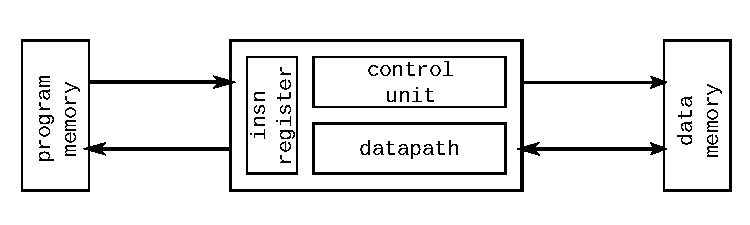
\includegraphics{../fig/processor.pdf}
	\caption{High level overview of the processor}
	\label{fig:processor}
\end{figure}
